% Copyright © 2013 Martin Ueding <dev@martin-ueding.de>
%
% Copyright © 2012-2013 Martin Ueding <dev@martin-ueding.de>

% This is my general purpose LaTeX header file for writing German documents.
% Ideally, you include this using a simple ``% Copyright © 2012-2013 Martin Ueding <dev@martin-ueding.de>

% This is my general purpose LaTeX header file for writing German documents.
% Ideally, you include this using a simple ``% Copyright © 2012-2013 Martin Ueding <dev@martin-ueding.de>

% This is my general purpose LaTeX header file for writing German documents.
% Ideally, you include this using a simple ``\input{header.tex}`` in your main
% document and start with ``\title`` and ``\begin{document}`` afterwards.

% If you need to add additional packages, I recommend not doing this in this
% file, but in your main document. That way, you can just drop in a new
% ``header.tex`` and get all the new commands without having to merge manually.

% Since this file encorporates a CC-BY-SA fragment, this whole files is
% licensed under the CC-BY-SA license.

\documentclass[11pt, ngerman, fleqn, DIV=15, headinclude]{scrartcl}

\usepackage{graphicx}

% Environment to quote the problem. Currently, this is just a new name for the
% quote environment.
\newenvironment{problem}{\begin{quote}}{\end{quote}}

%%%%%%%%%%%%%%%%%%%%%%%%%%%%%%%%%%%%%%%%%%%%%%%%%%%%%%%%%%%%%%%%%%%%%%%%%%%%%%%
%                                Locale, date                                 %
%%%%%%%%%%%%%%%%%%%%%%%%%%%%%%%%%%%%%%%%%%%%%%%%%%%%%%%%%%%%%%%%%%%%%%%%%%%%%%%

\usepackage{babel}
\usepackage[iso]{isodate}

%%%%%%%%%%%%%%%%%%%%%%%%%%%%%%%%%%%%%%%%%%%%%%%%%%%%%%%%%%%%%%%%%%%%%%%%%%%%%%%
%                          Margins and other spacing                          %
%%%%%%%%%%%%%%%%%%%%%%%%%%%%%%%%%%%%%%%%%%%%%%%%%%%%%%%%%%%%%%%%%%%%%%%%%%%%%%%

\usepackage[parfill]{parskip}
\usepackage{setspace}
\usepackage[activate]{microtype}

\setlength{\columnsep}{2cm}

%%%%%%%%%%%%%%%%%%%%%%%%%%%%%%%%%%%%%%%%%%%%%%%%%%%%%%%%%%%%%%%%%%%%%%%%%%%%%%%
%                                    Color                                    %
%%%%%%%%%%%%%%%%%%%%%%%%%%%%%%%%%%%%%%%%%%%%%%%%%%%%%%%%%%%%%%%%%%%%%%%%%%%%%%%

\usepackage[usenames, dvipsnames]{xcolor}

\colorlet{darkred}{red!70!black}
\colorlet{darkblue}{blue!70!black}
\colorlet{darkgreen}{green!40!black}

%%%%%%%%%%%%%%%%%%%%%%%%%%%%%%%%%%%%%%%%%%%%%%%%%%%%%%%%%%%%%%%%%%%%%%%%%%%%%%%
%                         Font and font like settings                         %
%%%%%%%%%%%%%%%%%%%%%%%%%%%%%%%%%%%%%%%%%%%%%%%%%%%%%%%%%%%%%%%%%%%%%%%%%%%%%%%

% This replaces all fonts with Bitstream Charter, Bitstream Vera Sans and
% Bitstream Vera Mono. Math will be rendered in Charter.
\usepackage[charter, greekuppercase=italicized]{mathdesign}
\usepackage{beramono}
\usepackage{berasans}

% Bold, sans-serif tensors. This fragment is taken from “egreg” from
% http://tex.stackexchange.com/a/82747/8945 and licensed under `CC-BY-SA
% <https://creativecommons.org/licenses/by-sa/3.0/>`_.
\usepackage{bm}
\DeclareMathAlphabet{\mathsfit}{\encodingdefault}{\sfdefault}{m}{sl}
\SetMathAlphabet{\mathsfit}{bold}{\encodingdefault}{\sfdefault}{bx}{sl}
\newcommand{\tens}[1]{\bm{\mathsfit{#1}}}

% Bold vectors.
\renewcommand{\vec}[1]{\boldsymbol{#1}}

%%%%%%%%%%%%%%%%%%%%%%%%%%%%%%%%%%%%%%%%%%%%%%%%%%%%%%%%%%%%%%%%%%%%%%%%%%%%%%%
%                               Input encoding                                %
%%%%%%%%%%%%%%%%%%%%%%%%%%%%%%%%%%%%%%%%%%%%%%%%%%%%%%%%%%%%%%%%%%%%%%%%%%%%%%%

\usepackage[T1]{fontenc}
\usepackage[utf8]{inputenc}

%%%%%%%%%%%%%%%%%%%%%%%%%%%%%%%%%%%%%%%%%%%%%%%%%%%%%%%%%%%%%%%%%%%%%%%%%%%%%%%
%                         Hyperrefs and PDF metadata                          %
%%%%%%%%%%%%%%%%%%%%%%%%%%%%%%%%%%%%%%%%%%%%%%%%%%%%%%%%%%%%%%%%%%%%%%%%%%%%%%%

\usepackage{hyperref}
\usepackage{lastpage}

% This sets the author in the properties of the PDF as well. If you want to
% change it, just override it with another ``\hypersetup`` call.
\hypersetup{
	breaklinks=false,
	citecolor=darkgreen,
	colorlinks=true,
	linkcolor=darkblue,
	menucolor=black,
	pdfauthor={Martin Ueding},
	urlcolor=darkblue,
}

%%%%%%%%%%%%%%%%%%%%%%%%%%%%%%%%%%%%%%%%%%%%%%%%%%%%%%%%%%%%%%%%%%%%%%%%%%%%%%%
%                               Math Operators                                %
%%%%%%%%%%%%%%%%%%%%%%%%%%%%%%%%%%%%%%%%%%%%%%%%%%%%%%%%%%%%%%%%%%%%%%%%%%%%%%%

% AMS environments like ``align`` and theorems like ``proof``.
\usepackage{amsmath}
\usepackage{amsthm}

% Common math constructs like partial derivatives.
\usepackage{commath}

% Physical units.
\usepackage[output-decimal-marker={,}]{siunitx}

% Word like operators.
\DeclareMathOperator{\acosh}{arcosh}
\DeclareMathOperator{\arcosh}{arcosh}
\DeclareMathOperator{\arcsinh}{arsinh}
\DeclareMathOperator{\arsinh}{arsinh}
\DeclareMathOperator{\asinh}{arsinh}
\DeclareMathOperator{\card}{card}
\DeclareMathOperator{\csch}{cshs}
\DeclareMathOperator{\diam}{diam}
\DeclareMathOperator{\sech}{sech}
\renewcommand{\Im}{\mathop{{}\mathrm{Im}}\nolimits}
\renewcommand{\Re}{\mathop{{}\mathrm{Re}}\nolimits}

% Fourier transform.
\DeclareMathOperator{\fourier}{\ensuremath{\mathcal{F}}}

% Roman versions of “e” and “i” to serve as Euler's number and the imaginary
% constant.
\newcommand{\ee}{\eup}
\newcommand{\eup}{\mathrm e}
\newcommand{\ii}{\iup}
\newcommand{\iup}{\mathrm i}

% Symbols for the various mathematical fields (natural numbers, integers,
% rational numbers, real numbers, complex numbers).
\newcommand{\C}{\ensuremath{\mathbb C}}
\newcommand{\N}{\ensuremath{\mathbb N}}
\newcommand{\Q}{\ensuremath{\mathbb Q}}
\newcommand{\R}{\ensuremath{\mathbb R}}
\newcommand{\Z}{\ensuremath{\mathbb Z}}

% Shape like operators.
\DeclareMathOperator{\dalambert}{\Box}
\DeclareMathOperator{\laplace}{\bigtriangleup}
\newcommand{\curl}{\vnabla \times}
\newcommand{\divergence}[1]{\inner{\vnabla}{#1}}
\newcommand{\vnabla}{\vec \nabla}

\newcommand{\half}{\frac 12}

% Unit vector (German „Einheitsvektor“).
\newcommand{\ev}{\hat{\vec e}}

% Scientific notation for large numbers.
\newcommand{\e}[1]{\cdot 10^{#1}}

% Mathematician's notation for the inner (scalar, dot) product.
\newcommand{\bracket}[1]{\left\langle #1 \right\rangle}
\newcommand{\inner}[2]{\bracket{#1, #2}}

% Placeholders.
\newcommand{\emesswert}{\del{\messwert \pm \messwert}}
\newcommand{\fehlt}{\textcolor{darkred}{Hier fehlen noch Inhalte.}}
\newcommand{\messwert}{\textcolor{blue}{\square}}
\newcommand{\punkte}{\phantom{xxxxx}}
\newcommand{\punktevon}[1]{\begin{flushright}/ #1\end{flushright}}

% Separator for equations on a single line.
\newcommand{\eqnsep}{,\quad}

% Quantum Mechanics
\newcommand{\braket}[2]{\left\langle #1 \left. \vphantom{#1 #2} \right| #2 \right\rangle}
\newcommand{\braopket}[3]{\left\langle #1 \left. \vphantom{#1 #2 #3} \right| #2 \left. \vphantom{#1 #2 #3} \right| #3 \right\rangle}
\newcommand{\bra}[1]{\left\langle #1 \right|}
\newcommand{\ketbra}[2]{\left| #1 \vphantom{#2} \right\rangle \left\langle #2  \vphantom{#1} \right|}
\newcommand{\ket}[1]{\left| #1 \right\rangle}

%%%%%%%%%%%%%%%%%%%%%%%%%%%%%%%%%%%%%%%%%%%%%%%%%%%%%%%%%%%%%%%%%%%%%%%%%%%%%%%
%                                  Headings                                   %
%%%%%%%%%%%%%%%%%%%%%%%%%%%%%%%%%%%%%%%%%%%%%%%%%%%%%%%%%%%%%%%%%%%%%%%%%%%%%%%

% This will set fancy headings to the top of the page. The page number will be
% accompanied by the total number of pages. That way, you will know if any page
% is missing.
%
% If you do not want this for your document, you can just use
% ``\pagestyle{plain}``.

\usepackage{scrpage2}

\pagestyle{scrheadings}
\automark{section}
\cfoot{\footnotesize{Seite \thepage\ / \pageref{LastPage}}}
\chead{}
\ihead{}
\ohead{\rightmark}
\setheadsepline{.4pt}

%%%%%%%%%%%%%%%%%%%%%%%%%%%%%%%%%%%%%%%%%%%%%%%%%%%%%%%%%%%%%%%%%%%%%%%%%%%%%%%
%                            Bibliography (BibTeX)                            %
%%%%%%%%%%%%%%%%%%%%%%%%%%%%%%%%%%%%%%%%%%%%%%%%%%%%%%%%%%%%%%%%%%%%%%%%%%%%%%%

\newcommand{\bibliographyfile}{../../zentrale_BibTeX/Central}
\bibliographystyle{apalike2}

%%%%%%%%%%%%%%%%%%%%%%%%%%%%%%%%%%%%%%%%%%%%%%%%%%%%%%%%%%%%%%%%%%%%%%%%%%%%%%%
%                                Abbreviations                                %
%%%%%%%%%%%%%%%%%%%%%%%%%%%%%%%%%%%%%%%%%%%%%%%%%%%%%%%%%%%%%%%%%%%%%%%%%%%%%%%

\newcommand{\dhabk}{\mbox{d.\,h.}}

%%%%%%%%%%%%%%%%%%%%%%%%%%%%%%%%%%%%%%%%%%%%%%%%%%%%%%%%%%%%%%%%%%%%%%%%%%%%%%%
%                                  Licences                                   %
%%%%%%%%%%%%%%%%%%%%%%%%%%%%%%%%%%%%%%%%%%%%%%%%%%%%%%%%%%%%%%%%%%%%%%%%%%%%%%%

\usepackage{ccicons}

\newcommand{\ccbysadetext}{%
	\begin{small}
		Dieses Werk bzw. Inhalt steht unter einer
		\href{http://creativecommons.org/licenses/by-sa/3.0/deed.de}{%
			Creative Commons Namensnennung - Weitergabe unter gleichen
		Bedingungen 3.0 Unported Lizenz}.
	\end{small}
}

\newcommand{\ccbysadetitle}{%
	Lizenz: \href{http://creativecommons.org/licenses/by-sa/3.0/deed.de}
	{CC-BY-SA 3.0 \ccbysa}
}
`` in your main
% document and start with ``\title`` and ``\begin{document}`` afterwards.

% If you need to add additional packages, I recommend not doing this in this
% file, but in your main document. That way, you can just drop in a new
% ``header.tex`` and get all the new commands without having to merge manually.

% Since this file encorporates a CC-BY-SA fragment, this whole files is
% licensed under the CC-BY-SA license.

\documentclass[11pt, ngerman, fleqn, DIV=15, headinclude]{scrartcl}

\usepackage{graphicx}

% Environment to quote the problem. Currently, this is just a new name for the
% quote environment.
\newenvironment{problem}{\begin{quote}}{\end{quote}}

%%%%%%%%%%%%%%%%%%%%%%%%%%%%%%%%%%%%%%%%%%%%%%%%%%%%%%%%%%%%%%%%%%%%%%%%%%%%%%%
%                                Locale, date                                 %
%%%%%%%%%%%%%%%%%%%%%%%%%%%%%%%%%%%%%%%%%%%%%%%%%%%%%%%%%%%%%%%%%%%%%%%%%%%%%%%

\usepackage{babel}
\usepackage[iso]{isodate}

%%%%%%%%%%%%%%%%%%%%%%%%%%%%%%%%%%%%%%%%%%%%%%%%%%%%%%%%%%%%%%%%%%%%%%%%%%%%%%%
%                          Margins and other spacing                          %
%%%%%%%%%%%%%%%%%%%%%%%%%%%%%%%%%%%%%%%%%%%%%%%%%%%%%%%%%%%%%%%%%%%%%%%%%%%%%%%

\usepackage[parfill]{parskip}
\usepackage{setspace}
\usepackage[activate]{microtype}

\setlength{\columnsep}{2cm}

%%%%%%%%%%%%%%%%%%%%%%%%%%%%%%%%%%%%%%%%%%%%%%%%%%%%%%%%%%%%%%%%%%%%%%%%%%%%%%%
%                                    Color                                    %
%%%%%%%%%%%%%%%%%%%%%%%%%%%%%%%%%%%%%%%%%%%%%%%%%%%%%%%%%%%%%%%%%%%%%%%%%%%%%%%

\usepackage[usenames, dvipsnames]{xcolor}

\colorlet{darkred}{red!70!black}
\colorlet{darkblue}{blue!70!black}
\colorlet{darkgreen}{green!40!black}

%%%%%%%%%%%%%%%%%%%%%%%%%%%%%%%%%%%%%%%%%%%%%%%%%%%%%%%%%%%%%%%%%%%%%%%%%%%%%%%
%                         Font and font like settings                         %
%%%%%%%%%%%%%%%%%%%%%%%%%%%%%%%%%%%%%%%%%%%%%%%%%%%%%%%%%%%%%%%%%%%%%%%%%%%%%%%

% This replaces all fonts with Bitstream Charter, Bitstream Vera Sans and
% Bitstream Vera Mono. Math will be rendered in Charter.
\usepackage[charter, greekuppercase=italicized]{mathdesign}
\usepackage{beramono}
\usepackage{berasans}

% Bold, sans-serif tensors. This fragment is taken from “egreg” from
% http://tex.stackexchange.com/a/82747/8945 and licensed under `CC-BY-SA
% <https://creativecommons.org/licenses/by-sa/3.0/>`_.
\usepackage{bm}
\DeclareMathAlphabet{\mathsfit}{\encodingdefault}{\sfdefault}{m}{sl}
\SetMathAlphabet{\mathsfit}{bold}{\encodingdefault}{\sfdefault}{bx}{sl}
\newcommand{\tens}[1]{\bm{\mathsfit{#1}}}

% Bold vectors.
\renewcommand{\vec}[1]{\boldsymbol{#1}}

%%%%%%%%%%%%%%%%%%%%%%%%%%%%%%%%%%%%%%%%%%%%%%%%%%%%%%%%%%%%%%%%%%%%%%%%%%%%%%%
%                               Input encoding                                %
%%%%%%%%%%%%%%%%%%%%%%%%%%%%%%%%%%%%%%%%%%%%%%%%%%%%%%%%%%%%%%%%%%%%%%%%%%%%%%%

\usepackage[T1]{fontenc}
\usepackage[utf8]{inputenc}

%%%%%%%%%%%%%%%%%%%%%%%%%%%%%%%%%%%%%%%%%%%%%%%%%%%%%%%%%%%%%%%%%%%%%%%%%%%%%%%
%                         Hyperrefs and PDF metadata                          %
%%%%%%%%%%%%%%%%%%%%%%%%%%%%%%%%%%%%%%%%%%%%%%%%%%%%%%%%%%%%%%%%%%%%%%%%%%%%%%%

\usepackage{hyperref}
\usepackage{lastpage}

% This sets the author in the properties of the PDF as well. If you want to
% change it, just override it with another ``\hypersetup`` call.
\hypersetup{
	breaklinks=false,
	citecolor=darkgreen,
	colorlinks=true,
	linkcolor=darkblue,
	menucolor=black,
	pdfauthor={Martin Ueding},
	urlcolor=darkblue,
}

%%%%%%%%%%%%%%%%%%%%%%%%%%%%%%%%%%%%%%%%%%%%%%%%%%%%%%%%%%%%%%%%%%%%%%%%%%%%%%%
%                               Math Operators                                %
%%%%%%%%%%%%%%%%%%%%%%%%%%%%%%%%%%%%%%%%%%%%%%%%%%%%%%%%%%%%%%%%%%%%%%%%%%%%%%%

% AMS environments like ``align`` and theorems like ``proof``.
\usepackage{amsmath}
\usepackage{amsthm}

% Common math constructs like partial derivatives.
\usepackage{commath}

% Physical units.
\usepackage[output-decimal-marker={,}]{siunitx}

% Word like operators.
\DeclareMathOperator{\acosh}{arcosh}
\DeclareMathOperator{\arcosh}{arcosh}
\DeclareMathOperator{\arcsinh}{arsinh}
\DeclareMathOperator{\arsinh}{arsinh}
\DeclareMathOperator{\asinh}{arsinh}
\DeclareMathOperator{\card}{card}
\DeclareMathOperator{\csch}{cshs}
\DeclareMathOperator{\diam}{diam}
\DeclareMathOperator{\sech}{sech}
\renewcommand{\Im}{\mathop{{}\mathrm{Im}}\nolimits}
\renewcommand{\Re}{\mathop{{}\mathrm{Re}}\nolimits}

% Fourier transform.
\DeclareMathOperator{\fourier}{\ensuremath{\mathcal{F}}}

% Roman versions of “e” and “i” to serve as Euler's number and the imaginary
% constant.
\newcommand{\ee}{\eup}
\newcommand{\eup}{\mathrm e}
\newcommand{\ii}{\iup}
\newcommand{\iup}{\mathrm i}

% Symbols for the various mathematical fields (natural numbers, integers,
% rational numbers, real numbers, complex numbers).
\newcommand{\C}{\ensuremath{\mathbb C}}
\newcommand{\N}{\ensuremath{\mathbb N}}
\newcommand{\Q}{\ensuremath{\mathbb Q}}
\newcommand{\R}{\ensuremath{\mathbb R}}
\newcommand{\Z}{\ensuremath{\mathbb Z}}

% Shape like operators.
\DeclareMathOperator{\dalambert}{\Box}
\DeclareMathOperator{\laplace}{\bigtriangleup}
\newcommand{\curl}{\vnabla \times}
\newcommand{\divergence}[1]{\inner{\vnabla}{#1}}
\newcommand{\vnabla}{\vec \nabla}

\newcommand{\half}{\frac 12}

% Unit vector (German „Einheitsvektor“).
\newcommand{\ev}{\hat{\vec e}}

% Scientific notation for large numbers.
\newcommand{\e}[1]{\cdot 10^{#1}}

% Mathematician's notation for the inner (scalar, dot) product.
\newcommand{\bracket}[1]{\left\langle #1 \right\rangle}
\newcommand{\inner}[2]{\bracket{#1, #2}}

% Placeholders.
\newcommand{\emesswert}{\del{\messwert \pm \messwert}}
\newcommand{\fehlt}{\textcolor{darkred}{Hier fehlen noch Inhalte.}}
\newcommand{\messwert}{\textcolor{blue}{\square}}
\newcommand{\punkte}{\phantom{xxxxx}}
\newcommand{\punktevon}[1]{\begin{flushright}/ #1\end{flushright}}

% Separator for equations on a single line.
\newcommand{\eqnsep}{,\quad}

% Quantum Mechanics
\newcommand{\braket}[2]{\left\langle #1 \left. \vphantom{#1 #2} \right| #2 \right\rangle}
\newcommand{\braopket}[3]{\left\langle #1 \left. \vphantom{#1 #2 #3} \right| #2 \left. \vphantom{#1 #2 #3} \right| #3 \right\rangle}
\newcommand{\bra}[1]{\left\langle #1 \right|}
\newcommand{\ketbra}[2]{\left| #1 \vphantom{#2} \right\rangle \left\langle #2  \vphantom{#1} \right|}
\newcommand{\ket}[1]{\left| #1 \right\rangle}

%%%%%%%%%%%%%%%%%%%%%%%%%%%%%%%%%%%%%%%%%%%%%%%%%%%%%%%%%%%%%%%%%%%%%%%%%%%%%%%
%                                  Headings                                   %
%%%%%%%%%%%%%%%%%%%%%%%%%%%%%%%%%%%%%%%%%%%%%%%%%%%%%%%%%%%%%%%%%%%%%%%%%%%%%%%

% This will set fancy headings to the top of the page. The page number will be
% accompanied by the total number of pages. That way, you will know if any page
% is missing.
%
% If you do not want this for your document, you can just use
% ``\pagestyle{plain}``.

\usepackage{scrpage2}

\pagestyle{scrheadings}
\automark{section}
\cfoot{\footnotesize{Seite \thepage\ / \pageref{LastPage}}}
\chead{}
\ihead{}
\ohead{\rightmark}
\setheadsepline{.4pt}

%%%%%%%%%%%%%%%%%%%%%%%%%%%%%%%%%%%%%%%%%%%%%%%%%%%%%%%%%%%%%%%%%%%%%%%%%%%%%%%
%                            Bibliography (BibTeX)                            %
%%%%%%%%%%%%%%%%%%%%%%%%%%%%%%%%%%%%%%%%%%%%%%%%%%%%%%%%%%%%%%%%%%%%%%%%%%%%%%%

\newcommand{\bibliographyfile}{../../zentrale_BibTeX/Central}
\bibliographystyle{apalike2}

%%%%%%%%%%%%%%%%%%%%%%%%%%%%%%%%%%%%%%%%%%%%%%%%%%%%%%%%%%%%%%%%%%%%%%%%%%%%%%%
%                                Abbreviations                                %
%%%%%%%%%%%%%%%%%%%%%%%%%%%%%%%%%%%%%%%%%%%%%%%%%%%%%%%%%%%%%%%%%%%%%%%%%%%%%%%

\newcommand{\dhabk}{\mbox{d.\,h.}}

%%%%%%%%%%%%%%%%%%%%%%%%%%%%%%%%%%%%%%%%%%%%%%%%%%%%%%%%%%%%%%%%%%%%%%%%%%%%%%%
%                                  Licences                                   %
%%%%%%%%%%%%%%%%%%%%%%%%%%%%%%%%%%%%%%%%%%%%%%%%%%%%%%%%%%%%%%%%%%%%%%%%%%%%%%%

\usepackage{ccicons}

\newcommand{\ccbysadetext}{%
	\begin{small}
		Dieses Werk bzw. Inhalt steht unter einer
		\href{http://creativecommons.org/licenses/by-sa/3.0/deed.de}{%
			Creative Commons Namensnennung - Weitergabe unter gleichen
		Bedingungen 3.0 Unported Lizenz}.
	\end{small}
}

\newcommand{\ccbysadetitle}{%
	Lizenz: \href{http://creativecommons.org/licenses/by-sa/3.0/deed.de}
	{CC-BY-SA 3.0 \ccbysa}
}
`` in your main
% document and start with ``\title`` and ``\begin{document}`` afterwards.

% If you need to add additional packages, I recommend not doing this in this
% file, but in your main document. That way, you can just drop in a new
% ``header.tex`` and get all the new commands without having to merge manually.

% Since this file encorporates a CC-BY-SA fragment, this whole files is
% licensed under the CC-BY-SA license.

\documentclass[11pt, ngerman, fleqn, DIV=15, headinclude]{scrartcl}

\usepackage{graphicx}

% Environment to quote the problem. Currently, this is just a new name for the
% quote environment.
\newenvironment{problem}{\begin{quote}}{\end{quote}}

%%%%%%%%%%%%%%%%%%%%%%%%%%%%%%%%%%%%%%%%%%%%%%%%%%%%%%%%%%%%%%%%%%%%%%%%%%%%%%%
%                                Locale, date                                 %
%%%%%%%%%%%%%%%%%%%%%%%%%%%%%%%%%%%%%%%%%%%%%%%%%%%%%%%%%%%%%%%%%%%%%%%%%%%%%%%

\usepackage{babel}
\usepackage[iso]{isodate}

%%%%%%%%%%%%%%%%%%%%%%%%%%%%%%%%%%%%%%%%%%%%%%%%%%%%%%%%%%%%%%%%%%%%%%%%%%%%%%%
%                          Margins and other spacing                          %
%%%%%%%%%%%%%%%%%%%%%%%%%%%%%%%%%%%%%%%%%%%%%%%%%%%%%%%%%%%%%%%%%%%%%%%%%%%%%%%

\usepackage[parfill]{parskip}
\usepackage{setspace}
\usepackage[activate]{microtype}

\setlength{\columnsep}{2cm}

%%%%%%%%%%%%%%%%%%%%%%%%%%%%%%%%%%%%%%%%%%%%%%%%%%%%%%%%%%%%%%%%%%%%%%%%%%%%%%%
%                                    Color                                    %
%%%%%%%%%%%%%%%%%%%%%%%%%%%%%%%%%%%%%%%%%%%%%%%%%%%%%%%%%%%%%%%%%%%%%%%%%%%%%%%

\usepackage[usenames, dvipsnames]{xcolor}

\colorlet{darkred}{red!70!black}
\colorlet{darkblue}{blue!70!black}
\colorlet{darkgreen}{green!40!black}

%%%%%%%%%%%%%%%%%%%%%%%%%%%%%%%%%%%%%%%%%%%%%%%%%%%%%%%%%%%%%%%%%%%%%%%%%%%%%%%
%                         Font and font like settings                         %
%%%%%%%%%%%%%%%%%%%%%%%%%%%%%%%%%%%%%%%%%%%%%%%%%%%%%%%%%%%%%%%%%%%%%%%%%%%%%%%

% This replaces all fonts with Bitstream Charter, Bitstream Vera Sans and
% Bitstream Vera Mono. Math will be rendered in Charter.
\usepackage[charter, greekuppercase=italicized]{mathdesign}
\usepackage{beramono}
\usepackage{berasans}

% Bold, sans-serif tensors. This fragment is taken from “egreg” from
% http://tex.stackexchange.com/a/82747/8945 and licensed under `CC-BY-SA
% <https://creativecommons.org/licenses/by-sa/3.0/>`_.
\usepackage{bm}
\DeclareMathAlphabet{\mathsfit}{\encodingdefault}{\sfdefault}{m}{sl}
\SetMathAlphabet{\mathsfit}{bold}{\encodingdefault}{\sfdefault}{bx}{sl}
\newcommand{\tens}[1]{\bm{\mathsfit{#1}}}

% Bold vectors.
\renewcommand{\vec}[1]{\boldsymbol{#1}}

%%%%%%%%%%%%%%%%%%%%%%%%%%%%%%%%%%%%%%%%%%%%%%%%%%%%%%%%%%%%%%%%%%%%%%%%%%%%%%%
%                               Input encoding                                %
%%%%%%%%%%%%%%%%%%%%%%%%%%%%%%%%%%%%%%%%%%%%%%%%%%%%%%%%%%%%%%%%%%%%%%%%%%%%%%%

\usepackage[T1]{fontenc}
\usepackage[utf8]{inputenc}

%%%%%%%%%%%%%%%%%%%%%%%%%%%%%%%%%%%%%%%%%%%%%%%%%%%%%%%%%%%%%%%%%%%%%%%%%%%%%%%
%                         Hyperrefs and PDF metadata                          %
%%%%%%%%%%%%%%%%%%%%%%%%%%%%%%%%%%%%%%%%%%%%%%%%%%%%%%%%%%%%%%%%%%%%%%%%%%%%%%%

\usepackage{hyperref}
\usepackage{lastpage}

% This sets the author in the properties of the PDF as well. If you want to
% change it, just override it with another ``\hypersetup`` call.
\hypersetup{
	breaklinks=false,
	citecolor=darkgreen,
	colorlinks=true,
	linkcolor=darkblue,
	menucolor=black,
	pdfauthor={Martin Ueding},
	urlcolor=darkblue,
}

%%%%%%%%%%%%%%%%%%%%%%%%%%%%%%%%%%%%%%%%%%%%%%%%%%%%%%%%%%%%%%%%%%%%%%%%%%%%%%%
%                               Math Operators                                %
%%%%%%%%%%%%%%%%%%%%%%%%%%%%%%%%%%%%%%%%%%%%%%%%%%%%%%%%%%%%%%%%%%%%%%%%%%%%%%%

% AMS environments like ``align`` and theorems like ``proof``.
\usepackage{amsmath}
\usepackage{amsthm}

% Common math constructs like partial derivatives.
\usepackage{commath}

% Physical units.
\usepackage[output-decimal-marker={,}]{siunitx}

% Word like operators.
\DeclareMathOperator{\acosh}{arcosh}
\DeclareMathOperator{\arcosh}{arcosh}
\DeclareMathOperator{\arcsinh}{arsinh}
\DeclareMathOperator{\arsinh}{arsinh}
\DeclareMathOperator{\asinh}{arsinh}
\DeclareMathOperator{\card}{card}
\DeclareMathOperator{\csch}{cshs}
\DeclareMathOperator{\diam}{diam}
\DeclareMathOperator{\sech}{sech}
\renewcommand{\Im}{\mathop{{}\mathrm{Im}}\nolimits}
\renewcommand{\Re}{\mathop{{}\mathrm{Re}}\nolimits}

% Fourier transform.
\DeclareMathOperator{\fourier}{\ensuremath{\mathcal{F}}}

% Roman versions of “e” and “i” to serve as Euler's number and the imaginary
% constant.
\newcommand{\ee}{\eup}
\newcommand{\eup}{\mathrm e}
\newcommand{\ii}{\iup}
\newcommand{\iup}{\mathrm i}

% Symbols for the various mathematical fields (natural numbers, integers,
% rational numbers, real numbers, complex numbers).
\newcommand{\C}{\ensuremath{\mathbb C}}
\newcommand{\N}{\ensuremath{\mathbb N}}
\newcommand{\Q}{\ensuremath{\mathbb Q}}
\newcommand{\R}{\ensuremath{\mathbb R}}
\newcommand{\Z}{\ensuremath{\mathbb Z}}

% Shape like operators.
\DeclareMathOperator{\dalambert}{\Box}
\DeclareMathOperator{\laplace}{\bigtriangleup}
\newcommand{\curl}{\vnabla \times}
\newcommand{\divergence}[1]{\inner{\vnabla}{#1}}
\newcommand{\vnabla}{\vec \nabla}

\newcommand{\half}{\frac 12}

% Unit vector (German „Einheitsvektor“).
\newcommand{\ev}{\hat{\vec e}}

% Scientific notation for large numbers.
\newcommand{\e}[1]{\cdot 10^{#1}}

% Mathematician's notation for the inner (scalar, dot) product.
\newcommand{\bracket}[1]{\left\langle #1 \right\rangle}
\newcommand{\inner}[2]{\bracket{#1, #2}}

% Placeholders.
\newcommand{\emesswert}{\del{\messwert \pm \messwert}}
\newcommand{\fehlt}{\textcolor{darkred}{Hier fehlen noch Inhalte.}}
\newcommand{\messwert}{\textcolor{blue}{\square}}
\newcommand{\punkte}{\phantom{xxxxx}}
\newcommand{\punktevon}[1]{\begin{flushright}/ #1\end{flushright}}

% Separator for equations on a single line.
\newcommand{\eqnsep}{,\quad}

% Quantum Mechanics
\newcommand{\braket}[2]{\left\langle #1 \left. \vphantom{#1 #2} \right| #2 \right\rangle}
\newcommand{\braopket}[3]{\left\langle #1 \left. \vphantom{#1 #2 #3} \right| #2 \left. \vphantom{#1 #2 #3} \right| #3 \right\rangle}
\newcommand{\bra}[1]{\left\langle #1 \right|}
\newcommand{\ketbra}[2]{\left| #1 \vphantom{#2} \right\rangle \left\langle #2  \vphantom{#1} \right|}
\newcommand{\ket}[1]{\left| #1 \right\rangle}

%%%%%%%%%%%%%%%%%%%%%%%%%%%%%%%%%%%%%%%%%%%%%%%%%%%%%%%%%%%%%%%%%%%%%%%%%%%%%%%
%                                  Headings                                   %
%%%%%%%%%%%%%%%%%%%%%%%%%%%%%%%%%%%%%%%%%%%%%%%%%%%%%%%%%%%%%%%%%%%%%%%%%%%%%%%

% This will set fancy headings to the top of the page. The page number will be
% accompanied by the total number of pages. That way, you will know if any page
% is missing.
%
% If you do not want this for your document, you can just use
% ``\pagestyle{plain}``.

\usepackage{scrpage2}

\pagestyle{scrheadings}
\automark{section}
\cfoot{\footnotesize{Seite \thepage\ / \pageref{LastPage}}}
\chead{}
\ihead{}
\ohead{\rightmark}
\setheadsepline{.4pt}

%%%%%%%%%%%%%%%%%%%%%%%%%%%%%%%%%%%%%%%%%%%%%%%%%%%%%%%%%%%%%%%%%%%%%%%%%%%%%%%
%                            Bibliography (BibTeX)                            %
%%%%%%%%%%%%%%%%%%%%%%%%%%%%%%%%%%%%%%%%%%%%%%%%%%%%%%%%%%%%%%%%%%%%%%%%%%%%%%%

\newcommand{\bibliographyfile}{../../zentrale_BibTeX/Central}
\bibliographystyle{apalike2}

%%%%%%%%%%%%%%%%%%%%%%%%%%%%%%%%%%%%%%%%%%%%%%%%%%%%%%%%%%%%%%%%%%%%%%%%%%%%%%%
%                                Abbreviations                                %
%%%%%%%%%%%%%%%%%%%%%%%%%%%%%%%%%%%%%%%%%%%%%%%%%%%%%%%%%%%%%%%%%%%%%%%%%%%%%%%

\newcommand{\dhabk}{\mbox{d.\,h.}}

%%%%%%%%%%%%%%%%%%%%%%%%%%%%%%%%%%%%%%%%%%%%%%%%%%%%%%%%%%%%%%%%%%%%%%%%%%%%%%%
%                                  Licences                                   %
%%%%%%%%%%%%%%%%%%%%%%%%%%%%%%%%%%%%%%%%%%%%%%%%%%%%%%%%%%%%%%%%%%%%%%%%%%%%%%%

\usepackage{ccicons}

\newcommand{\ccbysadetext}{%
	\begin{small}
		Dieses Werk bzw. Inhalt steht unter einer
		\href{http://creativecommons.org/licenses/by-sa/3.0/deed.de}{%
			Creative Commons Namensnennung - Weitergabe unter gleichen
		Bedingungen 3.0 Unported Lizenz}.
	\end{small}
}

\newcommand{\ccbysadetitle}{%
	Lizenz: \href{http://creativecommons.org/licenses/by-sa/3.0/deed.de}
	{CC-BY-SA 3.0 \ccbysa}
}


\usepackage{tikz}

\newcommand{\themodul}{physik411}
\newcommand{\thegruppe}{Gruppe 2}
\newcommand{\theuebung}{1}

\ifoot{\footnotesize{Martin Ueding}}
\ihead{\themodul{} -- Übung \theuebung}
\ofoot{\footnotesize{\thegruppe}}

\def\thesubsection{\thesection\alph{subsection}}

\title{\themodul{} -- Übung \theuebung \\ \vspace{0.5cm} \large{\thegruppe}}

\author{
	Martin Ueding \\ \small{\href{mailto:mu@uni-bonn.de}{mu@uni-bonn.de}}
}

\hypersetup{
	pdftitle={\themodul {} - Übung \theuebung},
}

\begin{document}

\maketitle

\begin{small}
	Symbolerklärung: Nabla $\vnabla$, Laplace $\laplace$, d'Alambert
	$\dalambert$, Delta $\Delta$ und $\Deltaup$, Vektor $\vec v$, Tensor $\tens
	T$.
\end{small}

\begin{table}[h]
	\centering
	\begin{tabular}{l|c|c|c|c|c|c}
		Aufgabe
		& \ref 1
		& \ref 2
		& \ref 3
		& \ref 4
		& \ref 5
		& $\sum$   \\
		\hline
		Punkte
		& \punkte / 8
		& \punkte / 12
		& \punkte / 5
		& \punkte / 9
		& \punkte / 9
		& \punkte / 43
	\end{tabular}
\end{table}

%%%%%%%%%%%%%%%%%%%%%%%%%%%%%%%%%%%%%%%%%%%%%%%%%%%%%%%%%%%%%%%%%%%%%%%%%%%%%%%
%                              Moleküle zählen                              %
%%%%%%%%%%%%%%%%%%%%%%%%%%%%%%%%%%%%%%%%%%%%%%%%%%%%%%%%%%%%%%%%%%%%%%%%%%%%%%%

\section{Moleküle zählen}

\label 1

\subsection{Wasserglas}

\SI{1}{mol} Wasser wiegt \SI{18}{g}. Dort drin sind \num{6.02e23} Moleküle
enthalten. Das Volumen ist \SI{18}{ml}. Im ganzen Glas sind also \num{6.69e24}
Moleküle enthalten. Da \SI{0.2}{l} nur eine signifikante Stelle hat, ist meine
Antwort \num{7e24} Moleküle.

\subsection{Markierung}

Zuerst schätze ich ab, welche Wassermenge der Planet hat. Dazu nehme ich an,
dass, wenn man die Meere gleichmäßig verteilt, sie eine Tiefe von vielleicht
\SI{1000}{m} haben. Das Volumen ist dann:
\[
	V = 4 \piup R_\text{E}^2 \cdot \SI{1000}{m}
	= \SI{5.15e17}{m^3}
\]

Geteilt durch die $\SI{18}{ml/mol} = \SI{1.8e-5}{m^3/mol}$ erhalte ich eine
Stoffmenge von \SI{2.86e22}{mol}, was \num{1.72e46} Teilchen entspricht.

Im Meer ist jetzt ein Anteil von \num{3.89e-22} Markiert. Wenn ich jetzt wieder
\num{6.69e24} Moleküle auswähle, dann ist der Erwartungswert \num{2600}
markierte Moleküle im Glas.

%%%%%%%%%%%%%%%%%%%%%%%%%%%%%%%%%%%%%%%%%%%%%%%%%%%%%%%%%%%%%%%%%%%%%%%%%%%%%%%
%                         Flugzeit-Massenspektrometer                         %
%%%%%%%%%%%%%%%%%%%%%%%%%%%%%%%%%%%%%%%%%%%%%%%%%%%%%%%%%%%%%%%%%%%%%%%%%%%%%%%

\section{Flugzeit-Massenspektrometer}

\label 2

\subsection{Skizze}

\begin{center}
	\begin{tikzpicture}
		\draw[dashed] (0, 0) -- ++(0, 3);
		\draw[dashed] (2, 0) -- ++(0, 3);
		\node[below] at (1, 0) {Kondensatorplatten};
		\draw[|-|] (0, 3.2) -- ++(2, 0) node[above, midway] {\SI{10}{mm}};
		\node[draw, rectangle, right] at (10, 1.5) {Detektor};
		\draw[|-|] (2, 3.2) -- (10, 3.2) node[above, midway] {\SI{1}{m}};
		\node[draw, circle] at (1, 1.5) {$\mathrm{NO}$};
	\end{tikzpicture}
\end{center}

\subsection{Flugzeit für $\mathrm{^{14}N^{16}O}$}

Die Masse des Isotops ist $\SI{30}{\atomicmassunit} = \SI{4.98e-26}{kg}$. Das
Ion legt eine Potentialdifferenz von \SI{500}{V} zurück (mittig im
Kondensator), es bekommt also $\SI{500}{eV} = \SI{8.05e-17}{J}$ Energie. Mit
$E_\text{kin} = mv^2/2$ erhalte ich eine Geschwindigkeit von $v =
\SI{56800}{m/s}$. Da die Ruhemasse im Bereich von \si{MeV} liegt, darf ich an
dieser Stelle klassisch rechnen. Mit dieser Geschwindigkeit $v$ legen die Ionen
die Strecke von $L = \SI1m$ in $t = \SI{1.76e-5}s$ zurück.

Dabei habe ich die Beschleunigungszeit nicht berücksichtigt. Das Ion
beschleunigt innerhalb von $d/2 = \SI5{mm}$ auf die Geschwindigkeit $v$. Mit
$v^2 = 2ad/2$ erhalte ich eine Beschleunigung von $a = \SI{3.23e11}{m/s^2}$.
Die Zeit, um diese Strecke zurück zu legen erhalte ich mit $d/2 = a \tilde
t^2/2$: $\tilde t = \SI{1.76e-7}s$. Der relative Fehler ist also \num{0.01}.

\subsection{Flugzeitverbreiterung}

Für die Flugzeitverbreiterung betrachte ich zwei Ionen, die an beiden Enden des
Wechselwirkungsgebietes gestartet sind. Die Ionen bekommen nun als Energie:
\[
	E_\pm = \frac{\frac d2 \pm \frac{\Deltaup x}2}d e U_0
\]

Diese Energien sind:
\[
	E_+ = \SI{8.13e-17}J
	\eqnsep
	E_- = \SI{7.96e-17}J
\]

Mit den eben benutzten Formeln errechne ich die Flugzeit für beide Ionen aus:
\[
	t_+ = \SI{1.75056e-5}s
	\eqnsep
	t_- = \SI{1.76815e-5}s
\]

Die Zeitauflösung ist also maximal \SI{1.759e-7}s, wenn die endliche Größe des
Wechselwirkungsgebietes berücksichtigt wird. Nun berechne ich die Flugzeit für
die verschiedenen Isotope, wenn sie aus der Mitte des Kondensators starten:
\begin{center}
	\begin{tabular}{lSSS}
		Isotop & {Masse / \si{\atomicmassunit}} & {Flugzeit $t$ / \si s} \\
		\hline
		$\mathrm{^{14}N^{16}O}$ & 30 & 1.75929e-5 \\
		$\mathrm{^{15}N^{16}O}$ & 31 & 1.78837e-5 \\
		$\mathrm{^{14}N^{18}O}$ & 32 & 1.81689e-5 \\
	\end{tabular}
\end{center}

Die Werte unterschieden sich mehr als \SI{2e-7}s, so dass eine Unterscheidung
möglich ist, wenn auch knapp.

%%%%%%%%%%%%%%%%%%%%%%%%%%%%%%%%%%%%%%%%%%%%%%%%%%%%%%%%%%%%%%%%%%%%%%%%%%%%%%%
%                          Mittlere freie Weglänge                           %
%%%%%%%%%%%%%%%%%%%%%%%%%%%%%%%%%%%%%%%%%%%%%%%%%%%%%%%%%%%%%%%%%%%%%%%%%%%%%%%

\section{Mittlere freie Weglänge}

\label 3

\subsection{Zimmerumgebung}

Gesucht ist die mittlere freie Weglänge $l$. Dazu stelle ich die Gasgleichung um:
\[
	pV = N k_\text{B}  T
	\iff
	p = n k_\text{B}  T
	\iff
	n = \frac p{k_\text{B} T}
\]

Die mittlere freie Weglänge $l$ ist:
\[
	l = \frac 1{n\sigma}
	\iff
	l = \frac{k_\text{B} T}{p\sigma}
	\implies
	l = \SI{1.00e-7}m
\]

Die Teilchendichte ist $n = \SI{2.50e25}{m^{-3}}$. Der mittlere Abstand $a$ zwischen den Teilchen ist dann:
\[
	a = \sqrt[3]{\frac 1n} = \SI{3.42e-9}m
\]

Dieser Abstand ist um zwei Größenordnungen kleiner als die mittlere freie
Weglänge. Dies liegt daran, dass der Wirkungsquerschnitt bei diesem Abstand
einen kleinen Raumwinkel einnimmt.

\subsection{Evakuieren}

Die gesuchte Teilchendichte ist $n = 1/l\sigma$. Nach der Gasgleichung ist dies auch gleich $p/k_\text{B} T$. Nach $p$ aufgelöst:
\[
	p = \frac{k_\text{B} T}{l \sigma} = \SI{10}{mPa}
\]

%%%%%%%%%%%%%%%%%%%%%%%%%%%%%%%%%%%%%%%%%%%%%%%%%%%%%%%%%%%%%%%%%%%%%%%%%%%%%%%
%                          De Broglie-Wellenlängen                           %
%%%%%%%%%%%%%%%%%%%%%%%%%%%%%%%%%%%%%%%%%%%%%%%%%%%%%%%%%%%%%%%%%%%%%%%%%%%%%%%

\section{De Broglie-Wellenlängen}

\label 4

\subsection{Energie \SI{10}{eV}}

Die Energie-Impuls-Relation besagt mit Gesamtenergie $E$, Ruheenergie $E_0$ und
Impuls $p$: $E^2 = E_0^2 + (cp)^2$. Die de Broglie-Wellenlänge eines Teilchens
ist $\lambda = h/p$. Damit errechne ich:
\[
	\lambda = \frac{ch}{\sqrt{\del{E_0 + \Deltaup E}^2 - E_0^2}}
\]

Dort setze ich $\Deltaup E = \SI{10}{eV}$ und $E_0 = \SI{511}{keV}$ ein und
erhalte $\lambda = \SI{3.86e-10}m$.

\subsection{Energie \SI{20}{keV}}

Gleiche Rechnung, nur mit anderer $\Deltaup E = \SI{20}{keV}$. Das Ergebnis ist
$\lambda = \SI{8.56}m$.

\subsection{$\alpha$-Teilchen}

Die Ruhemasse eines $\alpha$-Teilchens ist $m_\alpha = c^{-2} \cdot
\SI{3727}{MeV}$. Ich bestimme die Geschwindigkeit mit der relativistischen
Formel:
\[
	v = \SI{1.70e7}{m/s}
\]

\subsection{Stickstoffmolekül bei Zimmertemperatur}

Die Masse von $\mathrm{^{14}N_2}$ ist \SI{28}{\atomicmassunit}. Bei
Zimmertemperatur $T = \SI{290}{K}$ ist die kinetische Energie pro Freiheitsgrad
$E = kT/2$. Die mittlere Geschwindigkeit ist somit:
\[
	v
	= \sqrt{2 \frac Em}
	= \sqrt{\frac{kT}m}
	= \SI{293}{m/s}
\]

Der Impuls ist $p = \SI{1.37e-23}{kg.m/s}$, die de Broglie-Wellenlänge dazu ist
$\lambda = \SI{4.84e-11}{m}$.

Der Ablenkwinkel $\alpha$ für das erste Maximum ist mit der Formel aus der Optik:
\[
	\sin\del\alpha = \frac{\lambda}{a}
	\implies
	\alpha = \SI{484}{\micro rad}
\]

\subsection{Schnecke}

Das Gewicht einer Schnecke ist vielleicht $m = \SI{30}{g}$. Die
Kriechgeschwindigkeit ist vielleicht $v = \SI{1}{mm/s}$. Dann ist der Impuls $p
= mv = \SI{3.0e-5}{kg.m/s}$. Der Streuwinkel am Gitter mit $a = \SI{10}{cm}$
ist $\alpha = \SI{2.21e-28}{rad}$, also nicht zu beobachten.

Damit es aber überhaupt wirklich zur Interferenz kommen kann, darf der Ort der
Schnecke nicht mehr gemessen werden, bis sie durch den Gartenzaun ist. Dies ist
allerdings schwer möglich, da sie den Boden (der sie misst) zur Fortbewegung
braucht. Ohne Luft und Licht hat es die Schnecke noch schwerer.

\subsection{Photon}

Die Energie des Photons ist $E = ch/\lambda$. Sein Impuls ist $p = h/\lambda $.
Die de Broglie-Wellenlänge $\lambda_\text{dB}$ ist dann $\lambda$.

%%%%%%%%%%%%%%%%%%%%%%%%%%%%%%%%%%%%%%%%%%%%%%%%%%%%%%%%%%%%%%%%%%%%%%%%%%%%%%%
%                               Kastenpotential                               %
%%%%%%%%%%%%%%%%%%%%%%%%%%%%%%%%%%%%%%%%%%%%%%%%%%%%%%%%%%%%%%%%%%%%%%%%%%%%%%%

\section{Kastenpotential}

\label 5

Ich beginne mit der gegebenen Schrödingergleichung.
\begin{align*}
	\ii \hbar \partial_t \ket{\psi(x, t)} &= \hamilton \ket{\psi(x, t)} \\
	\ii \hbar \partial_t \ket{\psi(x, t)} &= \del{\frac{\hat p^2}{2m} + U(x)} \ket{\psi(x, t)} \\
	\intertext{%
		Der Impulsoperator $\hat p$ ist nach dem, was ich in \cite[Seite
		496]{penrose-road_to_reality} gelesen habe, $\hat p = \ii \hbar
		\partial_x$ und nicht proportional zu $\partial_t$. So kann ich die
		Schrödingergleichung schreiben als:
	}
	\ii \hbar \partial_t \ket{\psi(x, t)} &= \del{- \frac{\hbar^2}{2m} \partial_x^2 + U(x)} \ket{\psi(x, t)} \\
	\intertext{%
		Das Potential $U(x)$ ist innerhalb des kompakten Intervalls identisch
		null, so dass ich diesen Summanden weglassen kann, wenn ich das Problem
		nur auf diesem Intervall betrachte.
	}
	\ii \hbar \partial_t \ket{\psi(x, t)} &= -\frac{\hbar^2 }{2m} \partial_x^2 \ket{\psi(x, t)} &x \in \intcc{-\frac a2, \frac a2} \\
	\ii \partial_t \ket{\psi(x, t)} &= -\frac\hbar{2m} \partial_x^2 \ket{\psi(x, t)} &x \in \intcc{-\frac a2, \frac a2}
\end{align*}

Diese parabolische partielle Differentialgleichung auf einem kompakten
Intervall löse ich mit einem Separationsansatz. Mein Ansatz ist: $\psi(x, t) =
\phi(x) \theta(t)$. Damit wird die Gleichung zu:
\begin{align*}
	\ii \phi(x) \dot \theta(t) &= -\frac{\hbar^2}{2m} \phi''(x) \theta(t) &x \in \intcc{-\frac a2, \frac a2} \\
	\ii \frac{\dot \theta}\theta &= -\frac{\hbar^2}{2m} \frac{\phi''}\phi = \alpha^2 &x \in \intcc{-\frac a2, \frac a2}
\end{align*}

Die Integralbasis für $\phi$ besteht aus folgenden Elementen:
\[
	\set{
		\cos\del{\frac\hbar{\sqrt{2m}}\alpha x},
		\sin\del{\frac\hbar{\sqrt{2m}}\alpha x}
	}
\]

Die Integralbasis für $\theta$ dagegen ist:
\[
	\set{
		\exp\del{
			- \ii \alpha^2
		}
	}
\]

Das Teilchen darf sich außerhalb des Intervalls nicht aufhalten, da es dafür
dann eine unendliche Energie bräuchte. Daher muss die Wellenfunktion dort null
sein. Wegen der geforderten Stetigkeit von $\psi$ muss an den Randpunkten
$\psi\del{\pm a/2} = 0$ gelten.

Mit dieser Randbedingung kann ich nun $\alpha$ näher bestimmen. Es muss für den
Kosinus gelten:
\[
	\frac\hbar{\sqrt{2m}}\alpha \frac a2 = \del{n + \half} \piup
	\iff
	\alpha = \frac{(2n+1)\piup \sqrt{2m}}{a\hbar}
\]

Für den Sinus:
\[
	\frac\hbar{\sqrt{2m}}\alpha \frac a2 = n\piup
	\iff
	\alpha = \frac{2n\piup \sqrt{2m}}{a\hbar}
\]

Somit wird die Integralbasis für $\phi$ zu:
\[
	\set{
		\cos\del{\frac{(2n+1)\piup}{a} x},
		\sin\del{\frac{2n\piup}{a} x},
	}
\]

Das $\alpha$ für den Kosinus eingesetzt in die Integralbasis für $\theta$
liefert:
\[
	\set{
		\exp\del{
			- 2 \ii \frac{(2n+1)^2\piup^2 m}{a^2\hbar^2} t
		}
	}
\]

Für den Sinus geht dies analog.

\subsection{Mögliche Impulse}

Die Wellenzahlen $k$, die die Welle annehmen darf sind dann $n\piup/a$. Je nach
dem, ob es eine Sinus- oder Kosinuswelle ist, muss $n$ gerade beziehungsweise
ungerade sein.

\subsection{Energie der Welle}

Die Energie $E$ ist ein Eigenwert des Energieoperators $\iup \hbar \partial_t$.
Ich nehme mir den entsprechenden Teil aus der Schrödingergleichung:
\begin{align*}
	E \ket\psi &= \iup \hbar \partial_t \ket\psi \\
	\del{E - \ii \hbar \partial_t} \ket\psi &= 0 \\
	\del{E - \ii \hbar \partial_t} \cos(kx) \exp\del{- 2 \ii \frac{(2n+1)^2\piup^2 m}{a^2\hbar^2} t} &= 0
\end{align*}

Beim Ableiten nach der Zeit $t$ erhalte ich die innere Ableitung der Exponentialfunktion. Multipliziert mit dem Vorfaktor erhalte ich:
\[
	E = 2 \frac{(2n+1)^2\piup^2 m}{a^2\hbar}
\]

Von den Einheiten:
\[
	\si[per-mode=fraction]{\kilo\gram\per\meter\squared\per\joule\per\second}
	= \si[per-mode=fraction]{\kilo\gram\per\meter\squared\per\newton\per\meter\per\second}
	= \si[per-mode=fraction]{\kilo\gram\per\meter\cubed\per\newton\per\second}
	= \si[per-mode=fraction]{\kilo\gram\second\squared\per\meter\cubed\per\kilo\gram\per\meter\per\second}
	= \si[per-mode=fraction]{\second\per\meter\tothe 4}
\]

Da stimmt also etwas nicht, es sollte \si{N.m} herauskommen.

Jedenfalls lässt sich diese Rechnung noch für den Sinus wiederholen, die Energie ist dann für Bauchzahl $n$:
\[
	E = 2 \frac{n^2\piup^2 m}{a^2\hbar}
\]

\subsection{Normierung}

\begin{figure}[h!]
	\centering
	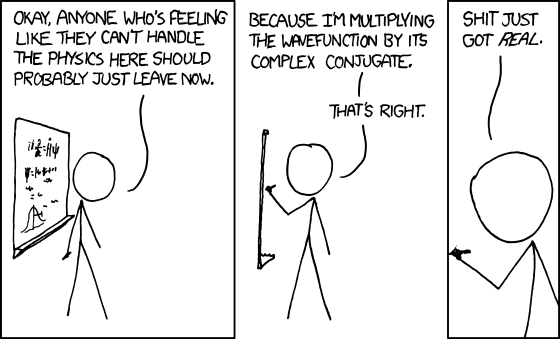
\includegraphics[width=.5\textwidth]{complex_conjugate.png}
	\caption{Bild aus \cite{xkcd-complex_conjugate}}
	\label{fig:}
\end{figure}

Die Normierung verlangt, dass gilt:
\begin{align*}
	\int_{-a/2}^{a/2} \dif x \, \braket{\phi(x, t)}{\phi(x, t)} &= 1 \\
	\intertext{%
		Das Argument der Exponentialfunktion in $\psi$ ist rein imaginär, so
		dass der Betrag gerade 1 ist. Diese kann ich hier weglassen.
	}
	\int_{-a/2}^{a/2} \dif x \, \psi_0^2 \cos^2\del{kx} &= 1 \\
	\intertext{%
		Ich wende die Potenzformel für den Kosinus an.
	}
	\int_{-a/2}^{a/2} \dif x \, \psi_0^2 \frac{1 + \cos\del{2kx}}{2} &= 1 \\
	\psi_0^2 \del{\frac a2 + \eval{\frac{1}{2k} \sin(2kx)}_{-a/2}^{a/2}} &= 1 \\
	\psi_0^2 \del{\frac a2 + \eval{\frac{1}{2k} \sin\del{\frac{2n\piup}{a}x}}_{-a/2}^{a/2}} &= 1 \\
	\psi_0^2 \del{\frac a2 + \frac{a}{(2+1)n\piup} \sin\del{\frac{(2n+1)\piup}2}} &= 1 \\
	\psi_0^2 \del{\frac a2 + \frac{a}{(2+1)n\piup}} &= 1 \\
	\psi_0^2 &= \del{\frac a2 + \frac{a}{(2+1)n\piup}}^{-1/2}  \\
\end{align*}

Somit ist die, für den Kosinus normierte, Wellenfunktion:
\[
	\psi(x, t) =
	\sum_n \beta_n
	\del{\frac a2 + \frac{a}{(2+1)n\piup}}^{-1/2}
	\cos\del{\frac{(2n+1)\piup}{a} x}
	\exp\del{- 2 \ii \frac{(2n+1)^2\piup^2 m}{a^2\hbar^2} t}
\]

Analog kann eine weitere Wellenfunktion mit dem Sinus aufgestellt werden.
Zusammen sind sie dann eine Fourierreihe der allgemeinen Lösung, die von den
Anfangsbedingungen abhängt.

%%%%%%%%%%%%%%%%%%%%%%%%%%%%%%%%%%%%%%%%%%%%%%%%%%%%%%%%%%%%%%%%%%%%%%%%%%%%%%%
%                                    Ende                                     %
%%%%%%%%%%%%%%%%%%%%%%%%%%%%%%%%%%%%%%%%%%%%%%%%%%%%%%%%%%%%%%%%%%%%%%%%%%%%%%%

\IfFileExists{\bibliographyfile}{
	\bibliography{\bibliographyfile}
}{}

\end{document}

% vim: spell spelllang=de
